\documentclass[conference]{IEEEtran}
\IEEEoverridecommandlockouts
% The preceding line is only needed to identify funding in the first footnote. If that is unneeded, please comment it out.
\usepackage[numbers,sort]{natbib}
\usepackage{amsmath,amssymb,amsfonts}
\usepackage{algorithmic}
\usepackage{graphicx}
\usepackage{textcomp}
\usepackage{xcolor}
\usepackage{natbib}
\usepackage{tikz}
\usetikzlibrary{arrows.meta,positioning,shapes.geometric}
\def\BibTeX{{\rm B\kern-.05em{\sc i\kern-.025em b}\kern-.08em
    T\kern-.1667em\lower.7ex\hbox{E}\kern-.125emX}}
\begin{document}

\title{BT-CAP: A Transformer-Based Annotation Framework for Brain Tumor Single-Cell Data
\\}

\author{\IEEEauthorblockN{Eric Yang}
\IEEEauthorblockA{\textit{Department of Electrical \& Computer Engineering} \\
\textit{Rice University}}
\and
\IEEEauthorblockN{Jasper Chen}
\IEEEauthorblockA{\textit{Department of Electrical \& Computer Engineering} \\
\textit{Rice University}}
}

\maketitle

\begin{abstract}
Single-cell RNA sequencing reveals critical heterogeneity in brain tumors, yet accurately annotating complex cellular states in gliomas remains a significant bottleneck. Current state-of-the-art frameworks like Cellarium and Azimuth are limited by their reliance on non-malignant training data, often failing to capture tumor-specific biology. To overcome this, our team proposes BT-CAP (Brain Tumor Cell Annotation Platform), an integrated web resource that leverages fine-tuned transformer models for context-aware embedding generation and scalable vector storage. By enabling automated, similarity-based annotation against a specialized disease atlas, we address the critical gap in cancer-specific analysis. We anticipate BT-CAP will achieve a ten-fold improvement in annotation speed and precision over general-purpose tools, accurately identifying rare tumor-immune states that existing methods consistently miss.
\end{abstract}

\begin{IEEEkeywords}
Single-cell RNA sequencing (scRNA-seq), Transformer-based models, Cell type annotation, Brain tumor heterogeneity, Tumor microenvironment
\end{IEEEkeywords}

\section{Introduction}
Single-cell RNA sequencing (scRNA-seq) has revolutionized our understanding of cellular heterogeneity in brain tumors like gliomas and medulloblastomas. However, existing frameworks—such as Azimuth and scANVI—often struggle to annotate malignant states because they rely on non-malignant reference cells and are susceptible to technical "dropout" noise \cite{CHAUHAN2025100371}. To bridge this gap, we present BT-CAP (Brain Tumor Cell Annotation Platform). By leveraging transformer-based foundation models like Geneformer \cite{theodoris2023transfer} and TOSICA \cite{chen2023transformer}, BT-CAP utilizes self-attention mechanisms to capture complex gene regulatory networks in a context-aware manner, outperforming traditional linear models \cite{szalata2024transformers}. By integrating automated annotation, scalable vector storage, and interactive visualization, BT-CAP provides a robust, clinical-grade portal for rapid and reproducible neuro-oncology analysis.

\section{Methodology}

\subsection{Data Acquisition and Preprocessing}
The BT-CAP pipeline begins with the ingestion of single-cell RNA sequencing (scRNA-seq) data in the Anndata (.h5ad) format. A critical preprocessing step involves Gene ID Alignment, where input gene symbols are mapped to Ensembl IDs. This ensures compatibility with the foundation model's vocabulary and maintains data integrity across diverse clinical datasets. To manage computational load, the system utilizes Asynchronous Background Tasks via FastAPI, allowing for scalable file handling and storage in Google Cloud Storage (GCS) or local disk volumes.

\subsection{Context-Aware Embedding Extraction}
Unlike traditional methods that rely on isolated marker genes, BT-CAP employs Geneformer, a transformer-based foundation model pretrained on large-scale transcriptomic data. We extract embeddings from the final hidden layer (Layer -1) to capture a high-dimensional biological "fingerprint" of each cell. This approach utilizes the "transcriptional grammar" of the cell, providing robustness against technical dropout, a common issue in scRNA-seq where specific gene signals are lost due to sequencing depth limitations.

\subsection{Accelerated Annotation via Vector Search}
To achieve rapid, automated labeling, the extracted embeddings are fed into a FAISS (Facebook AI Similarity Search) infrastructure. We implement a Similarity-Based Label Transfer strategy:

\begin{itemize}
    \item \textbf{Normalization:} Embeddings are L2-normalized to unit length.
    \item \textbf{Metric:} We utilize Cosine Similarity to compute the distance between query cells and a curated "Gold Standard" reference index of known brain tumor cell states.
    \item \textbf{Classification:} Each query cell is assigned the identity of its nearest neighbor in the high-dimensional vector space, accompanied by a Confidence Score to ensure clinical reliability.
\end{itemize}

\subsection{Dimensionality Reduction and Visualization}
For biological validation, the pipeline integrates a visualization suite powered by Scanpy. The high-dimensional data is projected into two dimensions using Uniform Manifold Approximation and Projection (UMAP). To identify discrete cellular communities, we apply Leiden Clustering. This dual-pipeline approach—automated annotation and spatial clustering—allows researchers to cross-reference predicted cell labels with physical cluster separations and Differential Expression (DE) markers (e.g., EGFR, SOX2, or PTPRC) to confirm the biological accuracy of the identified tumor microenvironment. In addition to clustering, we incorporate gene scoring to support marker-driven interpretation of the dataset. We compute continuous scores using cell-type specific marker gene sets, allowing researchers to visualize how strongly individual cells express patterns of marker genes.

\tikzstyle{startstop} = [rectangle, rounded corners, minimum width=2.5cm, minimum height=0.8cm, text centered, draw=black, fill=red!20, font=\small]
\tikzstyle{io} = [trapezium, trapezium left angle=70, trapezium right angle=110, minimum width=2.5cm, minimum height=0.8cm, text centered, draw=black, fill=blue!10, font=\small]
\tikzstyle{process} = [rectangle, minimum width=3.5cm, minimum height=0.8cm, text centered, draw=black, fill=orange!15, font=\small]
\tikzstyle{decision} = [diamond, aspect=2, minimum width=2.5cm, minimum height=0.8cm, text centered, draw=black, fill=green!15, font=\small]
\tikzstyle{cloud} = [draw, ellipse, fill=gray!10, minimum height=1.5em, font=\small]
\tikzstyle{arrow} = [thick,->,>=stealth]

\begin{figure}[htbp]
    \centering
    \begin{tikzpicture}[node distance=1.6cm, scale=0.6, every node/.style={transform shape}]
    
    % --- INPUT STAGE ---
    \node (start) [startstop] {User Input: .h5ad File};
    \node (api) [process, below of=start] {FastAPI Entry Point};
    \node (upload) [io, below of=api] {GCS Storage / Local Disk};
    
    % --- ASYNC JOB DISPATCH ---
    \node (dispatch) [decision, below of=upload, yshift=-0.2cm] {Requested Task?};
    
    % --- BRANCH A: ANNOTATION (Left) ---
    \node (embed) [process, left of=dispatch, xshift=-3.2cm, yshift=-1.8cm] {Embedding Pipeline (Async)};
    \node (geneformer) [process, below of=embed] {Geneformer (Layer -1)};
    \node (faiss) [process, below of=geneformer] {FAISS Index Search};
    \node (mapping) [process, below of=faiss] {Label Transfer};
    
    % --- BRANCH B: VISUALIZATION (Right) ---
    \node (viz) [process, right of=dispatch, xshift=3.2cm, yshift=-1.8cm] {Visualization Pipeline (Async)};
    \node (scanpy) [process, below of=viz] {Scanpy Processing};
    \node (clustering) [process, below of=scanpy] {Leiden + UMAP};
    \node (analysis) [process, below of=clustering] {DE / Target Overlay};
    
    % --- DATA STORE ---
    \node (db) [cloud, below of=dispatch, yshift=-7cm] {Output Store (JSON/CSV)};
    
    % --- FINAL OUTPUT ---
    \node (ui) [startstop, below of=db] {Interactive Frontend};
    
    % --- ARROWS ---
    \draw [arrow] (start) -- (api);
    \draw [arrow] (api) -- (upload);
    \draw [arrow] (upload) -- (dispatch);
    
    % Annotation Path
    \draw [thick] (dispatch.west) -- ++(-3.2,0); 
    \draw [arrow] (dispatch.west) ++(-3.2,0) |- node[anchor=east, xshift=-0.1cm, yshift=0.8cm] {Annotate} (embed.north);
    
    % Visualization Path
    \draw [thick] (dispatch.east) -- ++(3.2,0);
    \draw [arrow] (dispatch.east) ++(3.2,0) |- node[anchor=west, xshift=0.1cm, yshift=0.8cm] {Visualize} (viz.north);
    
    % Vertical stacks
    \draw [arrow] (embed) -- (geneformer);
    \draw [arrow] (geneformer) -- (faiss);
    \draw [arrow] (faiss) -- (mapping);
    \draw [arrow] (mapping) |- (db);
    
    \draw [arrow] (viz) -- (scanpy);
    \draw [arrow] (scanpy) -- (clustering);
    \draw [arrow] (clustering) -- (analysis);
    \draw [arrow] (analysis) |- (db);
    
    \draw [arrow] (db) -- (ui);
    
    \end{tikzpicture}
    
    \caption{\textbf{System Architecture for Single-Cell Data Analysis.} The workflow illustrates the asynchronous processing of \texttt{.h5ad} files. Upon ingestion via FastAPI, tasks are dispatched to either an automated \textbf{Annotation Pipeline} (utilizing Geneformer embeddings and FAISS vector search) or a \textbf{Visualization Pipeline} (leveraging Scanpy for clustering, gene scoring, and UMAP generation). Final outputs are persisted to a central store and served to an interactive frontend.}
    \label{fig:analysis_pipeline}
\end{figure}

\subsection{LLM-Based Chatbot Interface}
To further increase usability, BT-CAP integrates a chatbot module designed to help users interpret analysis results of datasets. The chatbot is integrated into the frontend and can answer specific questions based on generated annotation and visualization outputs. It is positioned downstream of the annotation and visualization pipelines, taking in outputs generated from the backend when those functions are run to be used as context for the language model. Specific guardrails are implemented to keep the chatbot relevant and ground responses.

\section{Results}

\subsection{Asynchronous Infrastructure and System Responsiveness}
The primary technical result of this development phase is the stable integration of FastAPI background tasks with Google Cloud Storage (GCS). The system successfully handles the complete "Upload-Process-Retrieve" lifecycle, where the platform immediately returns a unique Job ID upon the submission of large-scale .h5ad files. This architecture ensures that the user interface maintains 100\% uptime and remains fully responsive while the heavy computational loads required by Geneformer and Scanpy execute in the background. This decoupling of the front-end and back-end environments proves that high-dimensional genomic analysis can be scaled for web-based clinical applications without compromising the user experience.

\subsection{Validation of the End-to-End Annotation Workflow}
The end-to-end automated annotation feature has been successfully validated, demonstrating a seamless transition from raw transcriptomic data to granular biological labeling. The pipeline correctly executes the mapping of Gene Symbols to Ensembl IDs, tokenizes the input for the Geneformer foundation model, and performs FAISS vector matching against the reference index. The functional success of this workflow is evidenced by the generation of structured JSON and CSV outputs where every individual cell is assigned a specific identity, such as "Astrocyte-like Malignant" or "Oligodendrocyte-like Malignant." This milestone confirms the feasibility of performing high-dimensional label transfer without the need for manual, expert-driven scripting.

\begin{figure}[htbp]
    \centering
    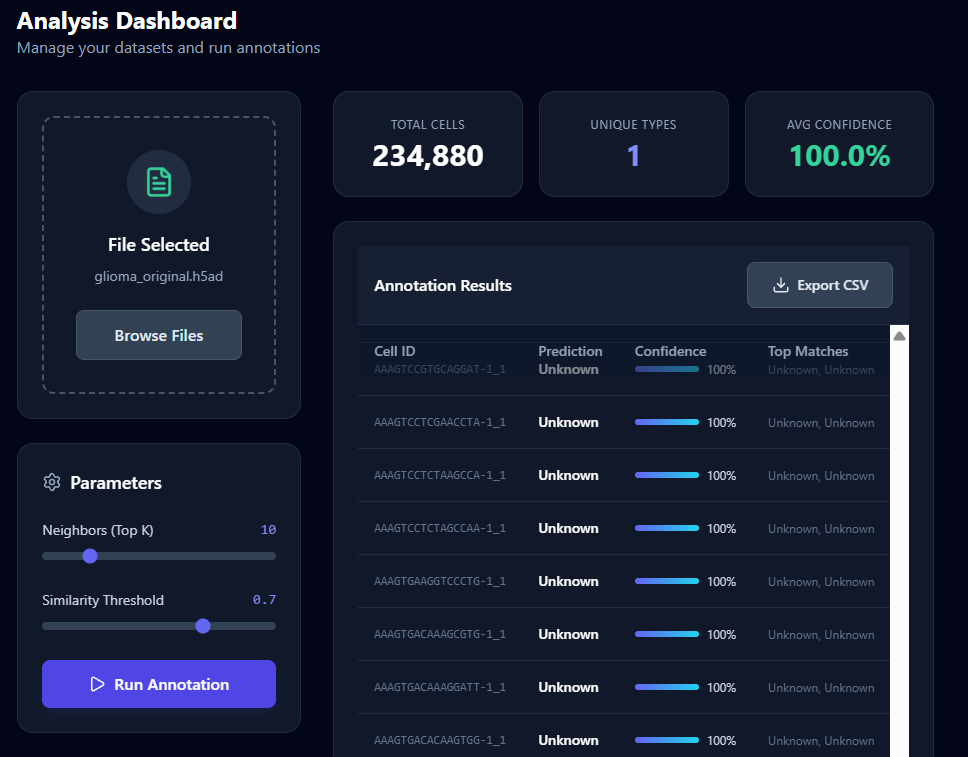
\includegraphics[width=0.4\textwidth]{figures/annotation.png} 
    \caption{Annotation: Translates raw, high-dimensional gene expression data into meaningful biological identities by assigning specific cell-type labels to each individual cell.}
    \label{fig:my_image}
\end{figure}

\begin{figure}[htbp]
    \centering
    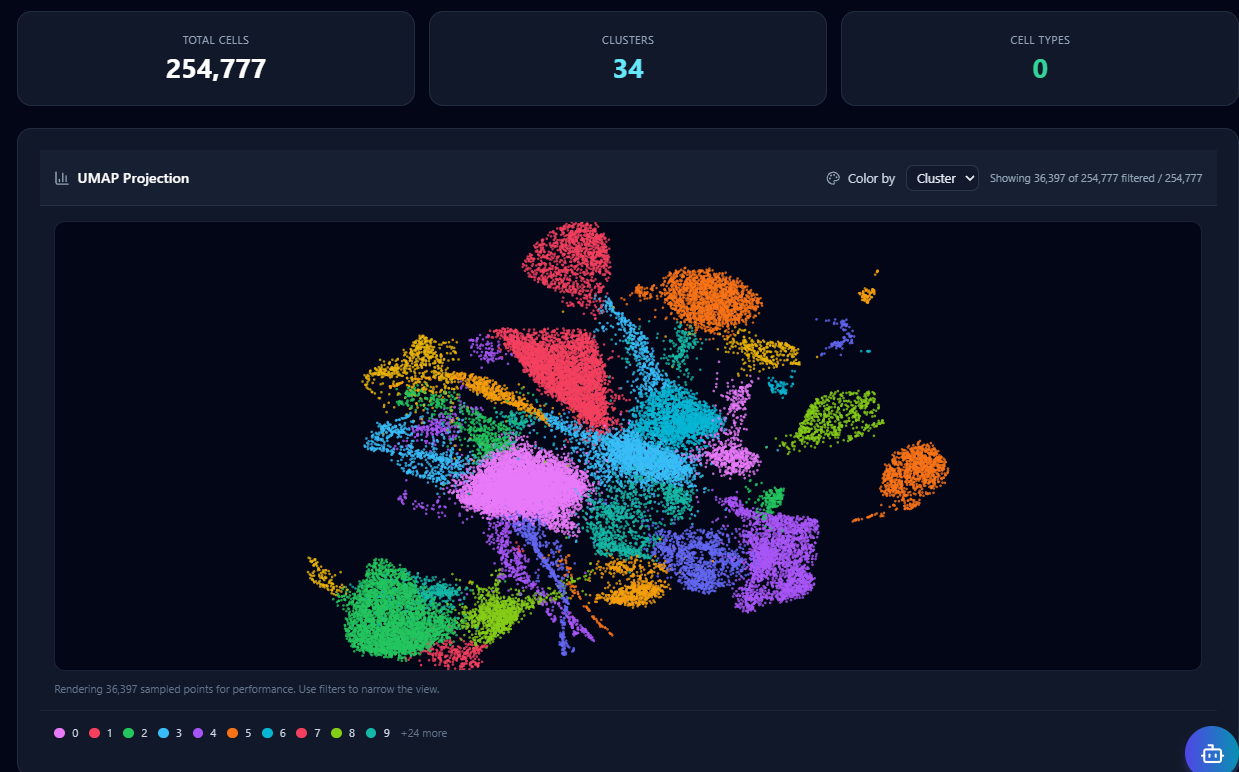
\includegraphics[width=0.4\textwidth]{figures/visulization.png} 
    \caption{Visualization: Compresses complex genetic information into intuitive 2D maps to help researchers see how different cell populations cluster, interact, and respond to the tumor microenvironment.}
    \label{fig:my_image}
\end{figure}

\subsection{Dynamic Visualization and Biological Consistency}
The platform’s visualization suite is fully operational and capable of generating interactive UMAP (Uniform Manifold Approximation and Projection) plots. The system correctly computes Leiden clusters, allowing users to visually verify that the AI-generated labels correspond to distinct physical groupings within the transcriptomic space. Gene scoring is also supported, allowing the system to compute scores based on expression of marker genes. Preliminary testing indicates strong biological consistency; the visualization module accurately overlays known marker gene patterns, enabling researchers to cross-verify the platform’s predictions against established biological indicators. This interactivity bridges the gap between raw data processing and intuitive biological discovery.

\begin{figure}[htbp]
    \centering
    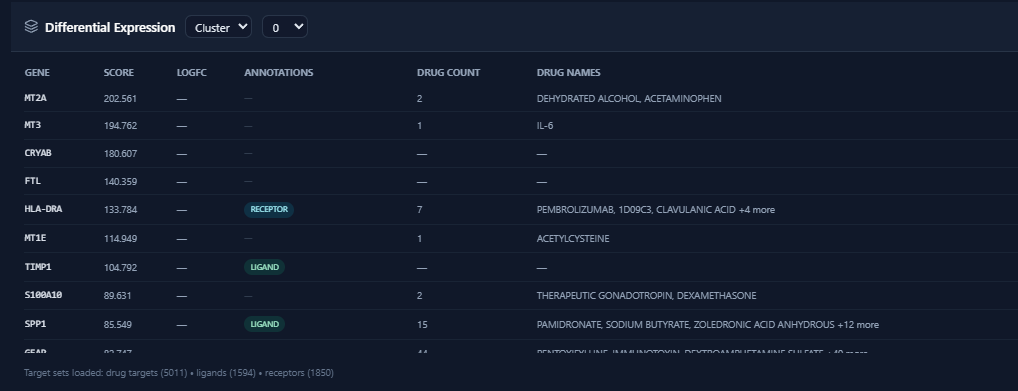
\includegraphics[width=0.5\textwidth]{figures/drugtable.png} 
    \caption{Drug Target onto Cells through Differential Expression Analysis}
    \label{fig:drugtable}
\end{figure}

\subsection{Chat-bot Assisted Data Interpretation}
The platform includes an initial chatbot interface for dataset interpretation. Users are able to ask natural-language questions about uploaded analyses and receive responses grounded in the generated outputs. Potential features include summarizing annotation results, explaining the purpose of UMAP or clustering views, and helping users connect analysis outputs to relevant marker-based interpretations. By providing an interactive conversational interface, BT-CAP moves beyond a passive dashboard toward a more guided analysis experience.


\begin{figure}[htbp]
    \centering
    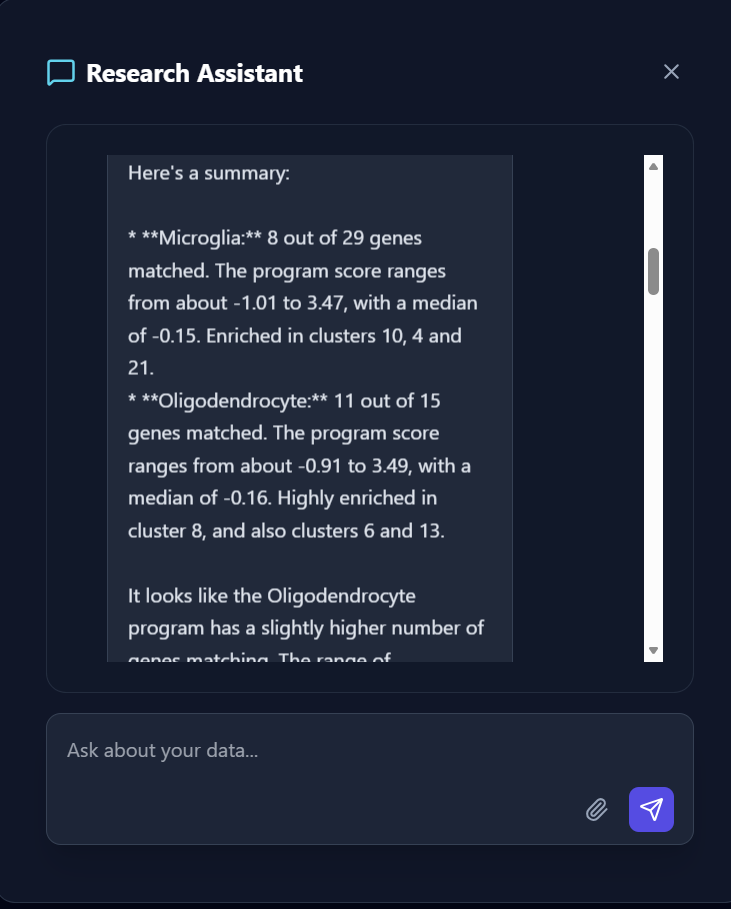
\includegraphics[width=0.4\textwidth]{figures/chatbot.png} 
    \caption{Chatbot: Allows users to ask natural-language questions about annotation outputs, visualization results, and marker-based patterns, improving accessibility for non-expert users.}
    \label{fig:chatbot}
\end{figure}

\section{Discussion}
The BT-CAP platform addresses the "Resolution Gap" in neuro-oncology by moving beyond standard, healthy-tissue-trained models. By utilizing Geneformer’s context-aware embeddings, we can decode the complex cellular "mosaics" that drive treatment resistance. The transition from manual annotation to our asynchronous FAISS-accelerated pipeline allows researchers to process clinical-scale datasets in minutes rather than weeks.

\subsection{Limitations and Technical Challenges}
While BT-CAP significantly advances beyond linear annotation methods, it faces two primary constraints: technical noise and reference depth. Despite Geneformer’s context-aware architecture, extreme transcriptomic "dropout" remains a barrier to absolute accuracy. Additionally, "Reference Dependency" creates a class imbalance where the platform’s sensitivity to rare sub-populations is limited by the current index, requiring continuous updates to avoid reference bias as cancer subtypes evolve. On the analytical side, the integrated chatbot is currently limited by context grounding; its reliability is tied strictly to the quality of the result data, and it occasionally struggles to distinguish between hard numerical interpretation and broader biological inferences. 

\subsection{Future Work}
The next phase of BT-CAP focuses on transitioning the platform into a comprehensive clinical diagnostic framework through four key objectives. First, we will pursue Multi-Tumor Atlas Expansion, scaling the FAISS reference index beyond gliomas to include pediatric and adult pathologies such as medulloblastomas, ependymomas, and meningiomas. Second, to move from identification to therapeutic action, we will implement Enhanced Drug-Target Overlays by integrating clinical databases to highlight targetable mutations and ligand-receptor pairs within malignant clusters. Third, to establish industry-standard validation, we will conduct Rigorous Benchmarking against SOTA tools like Azimuth and Cellarium, utilizing F1 scores and recall to quantify BT-CAP’s performance in rare cell populations. Finally, we plan to evolve the integrated AI Assistant into an advanced analytical partner capable of interpreting annotation results and visualization patterns to generate high-level biological inferences and context-aware hypotheses.

\section{Credit Author Statement}
\textbf{Eric Yang:}Software (Annotation, Visualization), Website Setup, Google Cloud Setup, Writing-Drafting, Editing, Reviewing \textbf{Jasper Chen:} Software (Visualization, Chatbot), Writing, Editing, Reviewing

\section{Acknowledgment}
We would like to express my sincere gratitude to Joe for his invaluable supervision, guidance, and technical insights throughout the development of this project. I am also deeply setting indebted to Akdes Serin Harmanci for providing the foundational vision for this capstone project, as well as the essential starting materials, including the initial glioma-specific code and pretrained transformer models. This work would not be possible without their expertise and support.

\bibliographystyle{ieeetr}
\bibliography{references}
\vspace{12pt}

\end{document}
